% ===== handout mode =====
% Comment/uncomment this line to toggle handout mode
% \newcommand{\handout}{}

% Comment/uncoment this line to toogle Mortitz mode
% \newcommand{\Moritz}{}

% Comment/uncomment this line to toggle handout mode
% \newcommand{\handout}{}

% by Stephan

%% Moritz mode or Stephan mode
\ifdefined \MoritzMode

% This is a configuration file with private, tutor specific information.
% It is therefore excluded from the Git repository so changes in this file will not conflict in git commits.

% Copy this Template, rename to config.tex and add your information below.

\newcommand{\mymail}{moritz.laupichler@student.kit.edu} % Consider using your named student Mail address to keep your u-Account private.

\newcommand{\myname}{\href{mailto:\mymail}{Moritz Laupichler}}

\newcommand{\mytutnumber}{27}

\newcommand{\mytutinfos}{Dienstags, 5. Block (15:45-17:15), SR 236}

\newcommand{\aboutMeFrame}{
	\begin{frame}{Euer Tutor}
		Name: \myname \\
		Alter: 19 Jahre \\
		Studiengang: Bachelor Informatik, 3. Semester \\
		\vspace{1cm}
		\pause 
		\centering{Kontakt: \href{mailto:\mymail}{\mymail}}
	\end{frame}
}

% Toggle Handout mode by including the following line before including style_tut
% and removing the % at the start (but do NOT remove it here, otherwise handout mode will always be on!)
% Please keep handout mode on in all commits!

% \newcommand{\handout}{} % Moritz mode
\fi
\ifdefined \AlexMode

% This is a configuration file with private, tutor specific information.
% It is therefore excluded from the Git repository so changes in this file will not conflict in git commits.

% Copy this Template, rename to config.tex and add your information below.

\newcommand{\mymail}{alexander.klug@student.kit.edu} % Consider using your named student Mail address to keep your u-Account private.

\newcommand{\myname}{\href{mailto:\mymail}{Alexander Klug}}

\newcommand{\mytutnumber}{30}

\newcommand{\mytutinfos}{Mittwochs, 3. Block (11:30-13:00), SR -107}

\newcommand{\aboutMeFrame}{
	\begin{frame}{Euer Tutor}
		Name: \myname \\
		Alter: 19 Jahre \\
		Studiengang: Bachelor Informatik, 3. Semester \\
		\vspace{1cm}
		\pause 
		\centering{Kontakt: \href{mailto:\mymail}{\mymail}}
	\end{frame}
}

% Toggle Handout mode by including the following line before including style_tut
% and removing the % at the start (but do NOT remove it here, otherwise handout mode will always be on!)
% Please keep handout mode on in all commits!

% \newcommand{\handout}{} % Alex Mode
\fi
\ifdefined \StephanMode

% This is a configuration file with private, tutor specific information.
% It is therefore excluded from the Git repository so changes in this file will not conflict in git commits.

% Copy this Template, rename to config.tex and add your information below.

\newcommand{\mymail}{stephan.bohr@student.kit.edu} % Consider using your named student Mail address to keep your u-Account private.

\newcommand{\myname}{\href{mailto:\mymail}{Stephan Bohr}}

\newcommand{\mytutnumber}{19}

\newcommand{\mytutinfos}{Dienstags, 3. Block (11:30-13:00), SR -108}

\newcommand{\aboutMeFrame}{
	\begin{frame}{Euer Tutor}
		Name: \myname \\
		Alter: 21 Jahre \\
		Studiengang: Bachelor Informatik, 5. Semester \\
		\vspace{1cm}
		\pause 
		\centering{Kontakt: \href{mailto:\mymail}{\mymail}}
	\end{frame}
} % Stephan mode
\fi

%% Beamer-Klasse im korrekten Modus
\ifdefined \handout
\documentclass[handout]{beamer} % Handout mode
\else
\documentclass{beamer}
\fi
%\documentclass[18pt,parskip]{beamer}

%% SLIDE FORMAT

% use 'beamerthemekit' for standard 4:3 ratio
% for widescreen slides (16:9), use 'beamerthemekitwide'

\usepackage{../templates/KIT-slides/beamerthemekit}
%\usepackage{../templates/KIT-slides/beamerthemekitwide}

%% TITLE PICTURE

% if a custom picture is to be used on the title page, copy it into the 'logos'
% directory, in the line below, replace 'mypicture' with the 
% filename (without extension) and uncomment the following line
% (picture proportions: 63 : 20 for standard, 169 : 40 for wide
% *.eps format if you use latex+dvips+ps2pdf, 
% *.jpg/*.png/*.pdf if you use pdflatex)

\titleimage{../figures/titleimage/brain}

%% TITLE LOGO

% for a custom logo on the front page, copy your file into the 'logos'
% directory, insert the filename in the line below and uncomment it

%\titlelogo{mylogo}

% (*.eps format if you use latex+dvips+ps2pdf,
% *.jpg/*.png/*.pdf if you use pdflatex)

%% TikZ INTEGRATION

% use these packages for PCM symbols and UML classes
% \usepackage{templates/tikzkit}
% \usepackage{templates/tikzuml}

%\usepackage{tikz}
%\usetikzlibrary{matrix}
%\usetikzlibrary{arrows.meta}
%\usetikzlibrary{automata}
%\usetikzlibrary{tikzmark}

%%%%%%%%%%%%%%%%%%%%%%%%%
% Libertine font (Original GBI font)
\usepackage[mono=false]{libertine}
%\renewcommand*\familydefault{\sfdefault}  %% Only if the base font of the document is to be sans serif

%% Schönere Schriften
\usepackage[TS1,T1]{fontenc}

%% Deutsche Silbentrennung und Beschriftungen
\usepackage[ngerman]{babel}

%% UTF-8-Encoding
\usepackage[utf8]{inputenc}

%% Bibliotheken für viele mathematische Symbole
\usepackage{amsmath, amsfonts, amssymb}

%% Anzeigetiefe für Inhaltsverzeichnis: 1 Stufe
\setcounter{tocdepth}{1}

%% Hyperlinks
\usepackage{hyperref}
% I don't know why, but this works and only includes sections and NOT subsections in the pdf-bookmarks.
\hypersetup{bookmarksdepth=subsection}

%% remove navigation symbols
\setbeamertemplate{navigation symbols}{}

%% switch between "ngerman" and "english" for German/English style date and logos
\selectlanguage{ngerman}

%% for invisible pause texts instead of dimming
\setbeamercovered{invisible}

\usepackage[german=swiss]{csquotes}

\usepackage{tabularx}
\usepackage{booktabs}

\usepackage{tikz}


% Problem: disabled itemize-icons
%\usepackage{enumitem}
% %\setlist[enumerate]{topsep=0pt,itemsep=-1ex,partopsep=1ex,parsep=1ex}
% \setlist[itemize]{noitemsep, nolistsep}
% \setlist[enumerate]{noitemsep, nolistsep}

% Mathmode no vertical space (https://tex.stackexchange.com/a/47403/146825)
\setlength{\abovedisplayskip}{0pt}
\setlength{\belowdisplayskip}{0pt}
\setlength{\abovedisplayshortskip}{0pt}
\setlength{\belowdisplayshortskip}{0pt}

%%%%%%%%%%%% Slides %%%%%%%%%%%%%%%%

\newcommand{\Moritz}[1]{
	\ifdefined \MoritzMode
	#1
	\fi
}

\newcommand{\Alex}[1]{
	\ifdefined \AlexMode
	#1
	\fi
}

\newcommand{\Stephan}[1]{
	\ifdefined \StephanMode
	#1
	\fi
}

\newcommand{\notMoritz}[1]{
	\Alex{#1} \Stephan{#1}
}

\newcommand{\notAlex}[1]{
	\Moritz{#1} \Stephan{#1}
}

\newcommand{\notStephan}[1]{
	\Alex{#1} \Moritz{#1}
}

%% Wochennummer
%\newcounter{weeknum}

%% Titelinformationen
%\title[GBI Tutorium, Woche \theweeknum]{Grundbegriffe der Informatik \\ Tutorium \mytutnumber}
%\subtitle{Termin \theweeknum \ | \mydate \\ \myname}
\author[\myname]{\myname}
\institute{Fakultät für Informatik}
%\date{\mydate}

%% Titel einfügen
\newcommand{\titleframe}{\frame{\titlepage}\addtocounter{framenumber}{-1}}


%% Alles starten mit \starttut{X}
%\newcommand{\starttut}[1]{\setcounter{weeknum}{#1}\titleframe\frame{\frametitle{Inhalt}\tableofcontents} \AtBeginSection[]{%
%\begin{frame}
%	\tableofcontents[currentsection]
%\end{frame}\addtocounter{framenumber}{-1}}}


%\newcommand{\framePrevEpisode}{
%	\begin{frame}
%		\centering
%		\textbf{In the previous episode of GBI...}
%	\end{frame}
%}

%% Roadmap frame
%table of contents
\newcommand{\roadmap}{
	\frame{\frametitle{Roadmap}\tableofcontents}}

 \AtBeginSection[]{%
\begin{frame}
	\frametitle{Roadmap}
	\tableofcontents[currentsection]
\end{frame}%\addtocounter{framenumber}{-1}
}


%% ShowMessage frame
\newcommand{\showmessage}[1]{\frame{\frametitle{\phantom{1em}}\centering\textbf{#1}}}

%% Fragen
%% Lastframe
\newcommand{\questionframe}{\showmessage{Fragen?}}

%% Lastframe
\newcommand{\lastframe}{\showmessage{Vielen Dank für Eure Aufmerksamkeit! \\Bis nächste Woche :)}}

%% Thanks frame
\newcommand{\slideThanks}{
	\begin{frame}
		\frametitle{Credits}
		\begin{block}{}
			An der Erstellung des Foliensatzes haben mitgewirkt:\\[1em]
			\Moritz{
			Stephan Bohr \\
			Alexander Klug \\
			}
			\Alex{
			Stephan Bohr \\
			Moritz Laupichler \\
			}
			\Stephan{
			Moritz Laupichler \\
			Alexander Klug \\
			}
			Katharina Wurz \\
			Thassilo Helmold \\
			Daniel Jungkind \\
			% Philipp Basler \\
			% Nils Braun \\
			% Dominik Doerner \\
			% Ou Yue \\
		\end{block}
	\end{frame}
}

%% Verbatim
%\usepackage{moreverb}

% GBI related stuff, but not beamer-stuff
\newcommand{\newpar}[1]{\paragraph{#1}\mbox{}\newline}

\newcommand{\nM}{\mathbb{M}}
\newcommand{\nR}{\mathbb{R}}
\newcommand{\nN}{\mathbb{N}}
\newcommand{\nZ}{\mathbb{Z}}
\newcommand{\nQ}{\mathbb{Q}}
\newcommand{\nB}{\mathbb{B}}
\newcommand{\nC}{\mathbb{C}}
\newcommand{\nK}{\mathbb{K}}
\newcommand{\nF}{\mathbb{F}}
\newcommand{\nG}{\mathbb{G}}
\newcommand{\nullel}{\mathcal{O}}
\newcommand{\einsel}{\mathds{1}}
\newcommand{\nP}{\mathbb{P}}
\newcommand{\Pot}{\mathcal{P}}
\renewcommand{\O}{\text{O}}

\newcommand{\bfmod}{\ensuremath{\text{\textbf{ mod }}}}
\renewcommand{\mod}{\bfmod}
\newcommand{\bfdiv}{\ensuremath{\text{\textbf{ div }}}}
\renewcommand{\div}{\bfdiv}


\newcommand{\set}[1]{\left\{ #1 \right\}}
\newcommand{\setc}[2]{\set{#1 \mid #2}}
\newcommand{\setC}[2]{\set{#1 \mid \text{ #2 }}}

\newcommand{\setsize}[1]{\; \mid #1 \mid \; }

\newcommand{\q}[1]{\textquotedblleft #1\textquotedblright}

% Zu zeigen, thx to http://www.matheboard.de/archive/155832/thread.html
\newcommand{\zz}{\ensuremath{\mathrm{z\kern-.29em\raise-0.44ex\hbox{z}}}:}

% Text above symbol
% https://tex.stackexchange.com/a/74132/146825
%
% \newcommand{\eqtext}[1]{\stackrel{\mathclap{\normalfont\mbox{#1}}}{=}}
% \newcommand{\gdwtext}[1]{\stackrel{\mathclap{\normalfont\mbox{#1}}}{\Leftrightarrow}}
% \newcommand{\imptext}[1]{\stackrel{\mathclap{\normalfont\mbox{#1}}}{\Rightarrow}}
% \newcommand{\symbtext}[2]{\stackrel{\mathclap{\normalfont\mbox{#2}}}{#1}}
\newcommand{\eqtext}[1]{\mathrel{\overset{\makebox%[0pt]
{\mbox{\normalfont\tiny #1}}}{=}}}
\newcommand{\gdwtext}[1]{\mathrel{\overset{\makebox%[0pt]
{\mbox{\normalfont\tiny #1}}}{\ensuremath{\Leftrightarrow}}}}
\newcommand{\imptext}[1]{\mathrel{\overset{\makebox%[0pt]
{\mbox{\normalfont\tiny #1}}}{\ensuremath{\Rightarrow}}}}
\newcommand{\symbtext}[2]{\mathrel{\overset{\makebox%[0pt]
{\mbox{\normalfont\tiny #2}}}{#1}}}

% qed symbol
\newcommand{\qedblack}{\hfill \ensuremath{\blacksquare}}
\newcommand{\qedwhite}{\hfill \ensuremath{\Box}}

% Aussagenlogik
% Worsch
\colorlet{alcolor}{blue}
\RequirePackage{tikz}
\usetikzlibrary{arrows.meta}
\newcommand{\alimpl}{\mathrel{\tikz[x={(0.1ex,0ex)},y={(0ex,0.1ex)},>={Classical TikZ Rightarrow[]}]{\draw[alcolor,->,line width=0.7pt,line cap=round] (0,0) -- (15,0);\path (0,-6);}}}
\newcommand{\alimp}{\alimpl}
\newcommand{\aleqv}{\mathrel{\tikz[x={(0.1ex,0ex)},y={(0ex,0.1ex)},>={Classical TikZ Rightarrow[]}]{\draw[alcolor,<->,line width=0.7pt,line cap=round] (0,0) -- (18,0);\path (0,-6);}}}
\newcommand{\aland}{\mathbin{\raisebox{-0.6pt}{\rotatebox{90}{\texttt{\color{alcolor}\char62}}}}}
\newcommand{\alor}{\mathbin{\raisebox{-0.8pt}{\rotatebox{90}{\texttt{\color{alcolor}\char60}}}}}
%\newcommand{\ali}[1]{_{\mathtt{\color{alcolor}#1}}}
\newcommand{\alv}[1]{\mathtt{\color{alcolor}#1}}
\newcommand{\alnot}{\mathop{\tikz[x={(0.1ex,0ex)},y={(0ex,0.1ex)}]{\draw[alcolor,line width=0.7pt,line cap=round,line join=round] (0,0) -- (10,0) -- (10,-4);\path (0,-8) ;}}}
\newcommand{\alP}{\alv{P}} %ali{#1}}
%\newcommand{\alka}{\negthinspace\hbox{\texttt{\color{alcolor}(}}}
\newcommand{\alka}{\negthinspace\text{\texttt{\color{alcolor}(}}}
%\newcommand{\alkz}{\texttt{\color{alcolor})}}\negthinspace}
\newcommand{\alkz}{\text{\texttt{\color{alcolor})}}\negthinspace}

% Thassilo
\newcommand{\BB}{\mathbb{B}}
\newcommand{\boder}{\alor}%{\ensuremath{\text{\;}\textcolor{blue}{\vee}}\text{\;}}
\newcommand{\bund}{\aland}%{\ensuremath{\text{\;}\textcolor{blue}{\wedge}}\text{\;}}
\newcommand{\bimp}{\alimp}%{\ensuremath{\text{\;}\textcolor{blue}{\to}}\text{\;}}
\newcommand{\bnot}{\alnot}%{\ensuremath{\text{\;}\textcolor{blue}{\neg}}\text{}}
\newcommand{\bgdw}{\aleqv}%{\ensuremath{\text{\;}\textcolor{blue}{\leftrightarrow}}\text{\;}}
\newcommand{\bone}{\ensuremath{\textcolor{blue}{1}}\text{}}
\newcommand{\bzero}{\ensuremath{\textcolor{blue}{0}}\text{}}
\newcommand{\bleftBr}{\alka}%{\ensuremath{\textcolor{blue}{(}}\text{}}
\newcommand{\brightBr}{\alkz}%{\ensuremath{\textcolor{blue}{)}}\text{}}

\newcommand{\val}{\hbox{\textit{val}}}

\newcommand{\VarAL}{\hbox{\textit{Var}}_{AL}}
\newcommand{\ForAL}{\hbox{\textit{For}}_{AL}}

% Validierungsfunktion val_i
\newcommand{\vali}[1]{\ensuremath{\val_I(#1)}}

% Boolsche Funktion b_
\newcommand{\bfnot}[1]{\ensuremath{b_{\bnot}(#1)}}
\newcommand{\bfand}[2]{\ensuremath{b_{\bund}(#1,#2)}}
\newcommand{\bfor}[2]{\ensuremath{b_{\boder}(#1,#2)}}
\newcommand{\bfimp}[2]{\ensuremath{b_{\bimp}(#1,#2)}}

% Aussagenkalkül
\newcommand{\AAL}{A_{AL}}
\newcommand{\LAL}{\hbox{\textit{For}}_{AL}}
\newcommand{\AxAL}{\hbox{\textit{Ax}}_{AL}}
\newcommand{\MP}{\hbox{\textit{MP}}}

% Prädikatenlogik
% die nachfolgenden Sachen angepasst an cmtt
\newlength{\ttquantwd}
\setlength{\ttquantwd}{1ex}
\newlength{\ttquantht}
\setlength{\ttquantht}{6.75pt}
\def\plall{%
  \tikz[line width=0.67pt,line cap=round,line join=round,baseline=(B),alcolor] {
    \draw (-0.5\ttquantwd,\ttquantht) -- node[coordinate,pos=0.4] (lll){} (-0.25pt,-0.0pt) -- (0.25pt,-0.0pt) -- node[coordinate,pos=0.6] (rrr){} (0.5\ttquantwd,\ttquantht);
    \draw (lll) -- (rrr);
    \coordinate (B) at (0,-0.35pt);
  }%
}
\def\plexist{%
  \tikz[line width=0.67pt,line cap=round,line join=round,baseline=(B),alcolor] {
    \draw (-0.9\ttquantwd,\ttquantht) -- (0,\ttquantht) -- node[coordinate,pos=0.5] (mmm){} (0,0) --  (-0.9\ttquantwd,0);
    \draw (mmm) -- ++(-0.75\ttquantwd,0);
    \coordinate (B) at (0,-0.35pt);
  }\ensuremath{\,}%
}
\let\plexists=\plexist
\newcommand{\NT}[1]{\ensuremath{\langle\mathrm{#1} \rangle}}
\newcommand{\CPL}{\text{\itshape Const}_{PL}}
\newcommand{\FPL}{\text{\itshape Fun}_{PL}}
\newcommand{\RPL}{\text{\itshape Rel}_{PL}}
\newcommand{\VPL}{\text{\itshape Var}_{PL}}
\newcommand{\plka}{\alka}
\newcommand{\plkz}{\alkz}
%\newcommand{\plka}{\plfoo{(}}
%\newcommand{\plkz}{\plfoo{)}}
\newcommand{\plcomma}{\hbox{\texttt{\color{alcolor},}}}
\newcommand{\pleq}{{\color{alcolor}\,\dot=\,}}

\newcommand{\plfoo}[1]{\mathtt{\color{alcolor}#1}}
\newcommand{\plc}{\plfoo{c}}
\newcommand{\pld}{\plfoo{d}}
\newcommand{\plf}{\plfoo{f}}
\newcommand{\plg}{\plfoo{g}}
\newcommand{\plh}{\plfoo{h}}
\newcommand{\plx}{\plfoo{x}}
\newcommand{\ply}{\plfoo{y}}
\newcommand{\plz}{\plfoo{z}}
\newcommand{\plR}{\plfoo{R}}
\newcommand{\plS}{\plfoo{S}}
\newcommand{\ar}{\mathrm{ar}}

\newcommand{\bv}{\mathrm{bv}}
\newcommand{\fv}{\mathrm{fv}}

\def\word#1{\hbox{\textcolor{blue}{\texttt{#1}}}}
%\let\literal\word
\def\mword#1{\hbox{\textcolor{blue}{$\mathtt{#1}$}}}  % math word
\def\sp{\scalebox{1}[.5]{\textvisiblespace}}
\def\wordsp{\word{\sp}}


\newcommand{\W}{\ensuremath{\hbox{\textbf{w}}}\xspace}
\newcommand{\F}{\ensuremath{\hbox{\textbf{f}}}\xspace}
\newcommand{\WF}{\ensuremath{\{\W,\F\}}\xspace}
\newcommand{\valDIb}{\val_{D,I,\beta}}

\newcommand{\impl}{\ifmmode\ensuremath{\mskip\thinmuskip\Rightarrow\mskip\thinmuskip}\else$\Rightarrow$\fi\xspace}
\newcommand{\Impl}{\ifmmode\implies\else$\Longrightarrow$\fi\xspace}

\newcommand{\derives}{\Rightarrow}

\newcommand{\gdw}{\ifmmode\mskip\thickmuskip\Leftrightarrow\mskip\thickmuskip\else$\Leftrightarrow$\fi\xspace}
\newcommand{\Gdw}{\ifmmode\iff\else$\Longleftrightarrow$\fi\xspace}

\newcommand*{\from}{\colon}
\newcommand{\functionto}{\longrightarrow}


\newcommand{\LTer}{L_{\text{\itshape Ter}}}
\newcommand{\LRel}{L_{\text{\itshape Rel}}}
\newcommand{\LFor}{L_{\text{\itshape For}}}
\newcommand{\NTer}{N_{\text{\itshape Ter}}}
\newcommand{\NRel}{N_{\text{\itshape Rel}}}
\newcommand{\NFor}{N_{\text{\itshape For}}}
\newcommand{\PTer}{P_{\text{\itshape Ter}}}
\newcommand{\PRel}{P_{\text{\itshape Rel}}}
\newcommand{\PFor}{P_{\text{\itshape For}}}

\newcommand{\sgn}{\mathop{\text{sgn}}}

\newcommand{\lang}[1]{\ensuremath{\langle#1\rangle}}

\newcommand{\literal}[1]{\hbox{\textcolor{blue!95!white}{\textup{\texttt{\scalebox{1.11}{#1}}}}}}
\let\hashtag\#
\renewcommand{\#}[1]{\literal{#1}}

\def\blank{\ensuremath{\openbox}}
\def\9{\blank}
\newcommand{\io}{\!\mid\!}


\providecommand{\fspace}{\mathord{\text{space}}}
\providecommand{\fSpace}{\mathord{\text{Space}}}
\providecommand{\ftime}{\mathord{\text{time}}}
\providecommand{\fTime}{\mathord{\text{Time}}}

\newcommand{\fnum}{\text{num}}
\newcommand{\fNum}{{\text{Num}}}

\def\Pclass{\text{\bfseries P}}
\def\PSPACE{\text{\bfseries PSPACE}}



\title[Mengen, Abbildungen, Relationen]{1. Tutorium\\ Mengen, Abbildungen, Relationen}
\subtitle{Grundbegriffe der Informatik, Tutorium \hashtag\mytutnumber}
\date{\today}

\begin{document}
\titleframe
\roadmap

%%%%%%%%%% %%%%%%%%%%
\section{Organisatorisches}
\subsection{Tutorium}

	\aboutMeFrame

	\Moritz{ 
		\showmessage{Und ihr?}
	}

	\begin{frame}{Infos zum Tutorium}
		\begin{itemize}
			\item Name: \myname
			\item Tutoriumsnummer: \mytutnumber
			\item \mytutinfos
		\end{itemize}	
	\end{frame}

	\begin{frame}{Infos zum Tutorium}
		Tutorium ist...\\
		\begin{itemize}
			\item Wiederholung der Vorlesung
			\item Gemeinsames Üben des aktuellen Stoffes
			\item Erste Anlaufstelle für Fragen
			\item Ausgabestelle der korrigierten Übungsblätter
		\end{itemize}
		\pause
		Tutorium ist nicht...\\
		\begin{itemize}
			\item Ersatz für die Vorlesung
			\item Lösen des kommenden Übungsblattes
		\end{itemize}
	\end{frame}
	
	\showmessage{Mitarbeit ist erwünscht!}
	
\subsection{Übungsblätter}
	\begin{frame}{Übungsblätter}
		\textbf{Ausgabe:} Mittwochs im ILIAS-Forum \\
		\pause
		\textbf{Abgabe:}
			\begin{itemize}
				\item Donnerstags, 16 Uhr, 2 Wochen nach Ausgabe
				\item richtiger Briefkasten im Infobau-UG (sortiert nach Tut.-Nummer)
				\pause
				\item \textbf{einzeln} und \textbf{handschriftlich} bearbeitet, Abschreiben führt zu Nichtbestehen des Scheines
				\item Blätter getackert
			\end{itemize}
		\pause	
		\textbf{Rückgabe:} Im Tutorium
	\end{frame}
\subsection{Schein/Klausur}
 \begin{frame}{Modul GBI}
		\textbf{Übungsschein}
			\begin{itemize}
				\item Erhält, wer mind. 50\% aller möglichen Punkte auf den Übungsblättern erzieht
				\item Ist keine Voraussetzung für die Teilnahme an der Klausur
				\item \textbf{Übungsschein wird zum Bestehen des Moduls benötigt} 
			\end{itemize}
		\pause	
		\textbf{Klausur}
		\begin{itemize}
				\item Datum: 08.03.18, 14-16 Uhr
				\item Nebenklausur nach dem SS
				\item Klausurnote = Modulnote
				\item \textbf{Klausur wird zum Bestehen des Moduls benötigt} 
			\end{itemize}
	\end{frame}
	
	\showmessage{Orientierungsprüfung!}


%\section[Nachrichten]{Nachrichten, Informationen}
%\subsection{}
	\begin{frame}
		\frametitle{Nachricht, Information, ...}
			\begin{block}{Nachricht}
			      Mitteilung, bei der vom Medium und den Einzelheiten der Signale abstrahiert wird.
			\end{block}
		\pause
			\begin{block}{Information}
		    	  Bedeutung, die einer Nachricht zugeordnet wird (kontextabhängig!).
			\end{block}
		\pause
			\begin{block}{Informationsgehalt}
				Anzahl der Elemente... \\
		     	Naturalis: log$_{e}$ \\
		      	Hartley: log$_{10}$ \\
		      	Shannon: log$_{2}$
		\end{block}
	\end{frame}

\section{Mengen}
\subsection{Basics}
	\begin{frame}{Mengen}
		\begin{block}{Def.: Menge}
			Eine \textbf{Menge} ist eine Zusammenfassung wohlunterschiedener Objekte zu einer Gesamtheit.\\
			Die leere Menge wird mit $\emptyset$ bezeichnet.\\
		\end{block}
		\pause
		\begin{exampleblock}{Beispiele}
			\begin{itemize}
				\item Aus der Schule kennen wir \qquad $\nN, \nZ, \nQ, \nR \qquad \nN_+, \nN_0$.
				\item Menge der natürlichen positiven Zahlen $\nN_+ = \{1,2,3,\dots\}$
				\item Menge d. Star-Wars-Filme: $\text{SW}:=\{4,5,6,1,2,3,7,\text{RO},8,\text{Solo}\} = \{1,2,3,\text{Solo},\text{RO},4,5,6,7,8\}$
				\item $\{1,1,2,3\} = \{1,2,3\}$
			\end{itemize}
		\end{exampleblock}
	\end{frame}

	\begin{frame}{Mengen}
		\begin{block}{Def.: Element}
			Ein Objekt $x$, dass in einer Menge $M$ enthalten ist, heißt \textbf{Element} von $M$. Man schreibt $x \in M$ (bzw. falls nicht: $x \notin M$).			
		\end{block}

		\begin{block}{Def.: Teilmenge}
			Sind alle Elemente einer Menge $A$ auch in einer Menge $B$ enthalten, so heißt $A$ \textbf{Teilmenge} von $B$. Man schreibt $A \subseteq B$.\\
			Es gilt für jede Menge $M$: $\emptyset \subseteq M$ und $M \subseteq M$.
		\end{block}
		\pause
		\begin{block}{set comprehension}
			Eine \textbf{set comprehension} ist eine Möglichkeit, eine Menge mit Bedingungen zu definieren:\\
			$\set{x \in \text{SW} \mid x \text{ ist vor 2010 erschienen}} = \set{1,2,3,4,5,6} \subseteq SW$.
		\end{block}
	\end{frame}

\subsection{Operationen}
	\begin{frame}{Mengen}
		\begin{block}{Def.: Kardinalität}
			Unter \textbf{Kardinalität} einer Menge $M$ versteht man die Anzahl der Elemente der Menge. Man schreibt $\setsize{M}$ .
		\end{block}
		\pause
		\begin{exampleblock}{Beispiele}
			\begin{itemize}
				\item $\setsize{SW} = \only<3->{10}$
				\item $\setsize{\emptyset} = \only<4->{0}$
				\item $\setsize{\{1,2,2,3\}} = \only<5->{3}$
				\item $\setsize{\set{1, 2, \set{}, \set{3,4}, \set{5, 6}}} = \only<6->{5}$
			\end{itemize}
		\end{exampleblock}
	\end{frame}

	\begin{frame}{Mengen}
		\begin{block}{Def.: Vereinigung}
			Die \textbf{Vereinigung} $A \cup B$ der Mengen $A$ und $B$ ist die Menge aller Elemente, die Elemente der Menge $A$ oder der Menge $B$ sind: $A \cup B = \{x \mid x \in A \text{ oder } x \in B\}$.
		\end{block}
		\pause
		\begin{exampleblock}{Beispiele}
			\begin{itemize}
				\item $\{1,3,5\}\cup\{2,4,6\} = \only<3->{\{1,2,3,4,5,6\}}$
				\item $\{4,5,6\}\cup\{1,2,3\}\cup\{7\}\cup\{RO\} = \only<4->{\{1,2,3,RO,4,5,6,7\}}$
				\item $\{1,2,3\}\cup\{2,3,4\} = \only<5->{\{1,2,3,4\}}$
				\item Für jede Menge $M$ gilt: $M \cup \emptyset = \only<6->{M}$
			\end{itemize}
		\end{exampleblock}
	\end{frame}

	\begin{frame}{Mengen}
		\begin{block}{Def.: Schnitt}
			Der (Durch-)\textbf{Schnitt} $A \cap B$ der Mengen $A$ und $B$ ist die Menge aller Elemente, die sowohl Elemente der Menge $A$ als auch der Menge $B$ sind: $A \cap B = \{x \mid x \in A \text{ und } x \in B\}$.\\
			Zwei Mengen heißen \textbf{disjunkt}, wenn ihr Schnitt leer ist, also $A \cap B = \emptyset$
		\end{block}
		\pause
		\begin{exampleblock}{Beispiele}
			\begin{itemize}
				\item $\{1,2,3\}\cap\{1,2\} = \only<3->{\{1,2\}}$
				\item $\set{1,2,3} \cap \set{3,4,5} = \only<4->{\set{3}}$
				\item $\set{a,b} \cap \set{x,y} = $ \only<5->{$\emptyset$ \quad (also sind $\set{a,b}$ und $\set{x,y}$ disjunkt)}
				\item Für jede Menge $M$ gilt: $M \cap \emptyset = \only<6->{\emptyset}$
			\end{itemize}
		\end{exampleblock}
	\end{frame}	

	\begin{frame}{Mengen}
		\begin{block}{Def.: Differenz}
			Die \textbf{Differenz} der Mengen $A$ und $B$ sind die Elemente, die in $A$ sind, aber nicht in $B$.
			$$A \setminus B = \{x \mid x \in A \text{ und } x \notin B\}$$
		\end{block}		
		\pause
		\begin{exampleblock}{Beispiele}
			\begin{itemize}
				\item $\set{1,2,3}\setminus\set{1} = \only<3->{\set{2,3}}$
				\item $\set{1,2,3}\setminus\set{4} = \only<4->{\set{1,2,3}}$
				\item $\set{1,2,3}\setminus\set{1,2,3,4,5,6} = \only<4->{\emptyset}$
				\item $\emptyset \setminus \set{a,b,c} = \only<5->{\emptyset}$
			\end{itemize}
		\end{exampleblock}
	\end{frame}

	\begin{frame}{Mengen}
	\begin{exampleblock}{Aufgabe}
		Seien $A = \{1, 2\}, B = \{3\}, C = \{1, 3\}  \subseteq M = \{1, 2, 3\}$ Mengen.\\
		Berechne folgende Mengen:
		\begin{align*}
		A \cup B &= \visible<2->{ \{1, 2, 3\} }  \\
		A \cap C &= \visible<3->{ \{1\} }\\
		A \setminus C &= \visible<4->{ \{2\} }\\
		B \setminus A &= \visible<5->{ \{3\} }\\
		A \cup (B \setminus C) &= \visible<6->{ \{1, 2\} }\\
		(A \setminus C) \cup B &= \visible<7->{ \{2, 3\} }\\
		A \cap B &= \visible<8->{ \emptyset }
		\end{align*}
	\end{exampleblock}
\end{frame}

\subsection{Mit Mengen umgehen}
	\begin{frame}{Mengen}
		Es gelten das Assoziativ- \\
			\begin{itemize}
				\item $(A\cup B) \cup C=A\cup(B\cup C)$
				\item $(A\cap B) \cap C=A\cap(B\cap C)$
			\end{itemize}
		und Distributivgesetz:\\
			\begin{itemize}
				\item $A\cup(B \cap C)=(A\cup B)\cap (A\cup C)$
				\item $A\cap(B \cup C)=(A\cap B)\cup (A\cap C)$
			\end{itemize}
	\end{frame}

	\begin{frame}{Mengen}
		\begin{block}{Def.: Potenzmenge}
		Die \textbf{Potenzmenge} $2^M$ oder auch $\Pot (M)$ ist die Menge aller möglicher Teilmengen von $M$. Es gilt also 
		\begin{align*}
			2^M = \{N \mid N \subseteq M\}
		\end{align*}
		\end{block}
		\pause
		\begin{exampleblock}{Beispiel}
		Betrachten wir nun   $M = \left\{ 1,2,0 \right\} $. \\
		Dann gilt 
		\begin{align*}
		2^M &= \left\{ \emptyset, \left\{ 0 \right\}, \left\{ 1 \right\}, \left\{ 2 \right\}, \left\{ 0,1 \right\} , \left\{ 0,2 \right\}, \left\{ 1,2 \right\}, \left\{ 0,1,2 \right\} \right\}
		\end{align*}
		
		Beachte: Es gilt immer $M \in 2^M \ \text{und} \ \emptyset \in 2^M$
		\end{exampleblock}
	\end{frame}

	\begin{frame}{Mengen}
		\begin{exampleblock}{Aufgabe}
		Es sei $M := \set{2,fish, 5}$. Bilde $\Pot (M)$. \\
		\pause
		$$\Pot (M) = \set{\emptyset, \set{2}, \set{fish}, \set{5}, \set{2,fish}, \set{2, 5}, \set{fish, 5}, \set{2,fish, 5}}$$
		\end{exampleblock}
		\pause
		\begin{exampleblock}{Aufgabe}
		Wie viele Elemente enthält $\Pot (M)$? \\
		\pause
		$$2^{\setsize{M}}$$
		\end{exampleblock}
	\end{frame}

	\begin{frame}{Mengen}
	\small{
		\begin{exampleblock}{Aufgabe}
			Es sei M eine Menge und es seien $A \subseteq M$ und $B \subseteq M$. Zeigen Sie: \\
			\centering $M \setminus (A \cup B) = (M \setminus A)  \cap (M \setminus B)$
		\end{exampleblock}
		}
	\pause 
	\tiny{
		\begin{block}{Lösung}
			$\subseteq$:
				Es sei $x \in M \setminus (A \cup B)$. Dann ist $x \in M$ und $x \notin (A \cup B)$.\\
				Also ist $x \notin A$ und $x \notin B$, womit:
				\begin{itemize}
					\itemsep0pt
					\item $x \in M$ und $x \notin A$ $\Longleftrightarrow $ $x \in M \setminus A$
					\item $x \in M$ und $x \notin B$ $\Longleftrightarrow$ $x \in M \setminus B$
				\end{itemize}
				Folglich ist $x \in (M \setminus A)  \cap (M \setminus B)$ \\

			\pause

			$\supseteq$:
				Es sei $x \in (M \setminus A) \cap (M \setminus B)$. Also gilt:
				\begin{itemize}
					\itemsep0pt
					\item $x \in M \setminus A$ $\Longleftrightarrow$ $x \in M$ und $x \notin A$
					\item $x \in M \setminus B$ $\Longleftrightarrow$ $x \in M$ und $x \notin B$
				\end{itemize}
				Damit ist $x \in M$, $x \notin A$ und $x \notin B$. \\
				Dies ist äquivalent zu $x \in M$ und $x \notin A \cup B$.
				Folglich ist $x \in M \setminus (A \cup B)$.

		\end{block}
		}
	\end{frame}

\section{Relationen}
\subsection{Tupel und Paare}

	\begin{frame}{Relationen}
		\begin{block}{Def.: Tupel bzw. Paare}
			Ein n-\textbf{Tupel} ist eine Liste von n Elementen. Die Reihenfolge ist dabei wichtig!\\
			Ein \textbf{Paar} ist ein Tupel der Länge 2, also ein 2-Tupel.			
		\end{block}
		\begin{exampleblock}{Beispiele:}
			\begin{itemize}
				\item Paare: $(1,2),(5,3),(Apfel, Birne)$
				\item 3-Tupel: $(1,2,3)$, 4-Tupel: $(4,3,2,1)$, ...
				\item $\set{1,2}=\set{2,1}$, aber $(1,2)\neq(2,1)$
			\end{itemize}			
		\end{exampleblock}	
	\end{frame}

	\begin{frame}{Relationen}
		\begin{block}{Def.: Kartesisches Produkt}
			Das \textbf{kartesische Produkt $A \times B$} der Mengen A und B ist die Menge aller Paare (a,b) mit $a \in A$ und $b \in B$, also:
			$$A \times B = \setC{(a,b)}{$a \in A$ und $b \in B$}$$
		\end{block}
	
		\begin{exampleblock}{Beispiele:}
			\begin{itemize}
				\item $\set{*, +} \times \set{1, 2, 3} = \set{(*,1), (*,2), (*,3), (+,1), (+,2), (+,3)}$
				\item $\set{0,1}^2 = \set{(0,0),(0,1),(1,0),(1,1)}$ 
				\item Für $A \neq B$ gilt im Allgemeinen: $A \times B \neq B \times A$
				\item Ist $A = \emptyset$ oder $B = \emptyset$, so gilt $A \times B = B \times A = \emptyset$
			\end{itemize}			
		\end{exampleblock}
	\end{frame}
%subsection Tupel und Paare (end)	
\subsection{Relationen}
	\begin{frame}{Relationen}
		\begin{block}{Def.: Relationen}
			Eine \textbf{binäre Relation R zwischen A und B} ist eine Teilmenge des kartesischen Produktes $A \times B$, also $R \subseteq A \times B$.\\
			Ist $A=B$, so heißt R eine Relation auf A.\\
			Erfüllt $(a,b) \in A \times B$ die Relation R, so schreibt man $(a,b) \in R$ oder $aRb$.
		\end{block}
	
		\begin{exampleblock}{Beispiele}
			\begin{itemize}
				\item Es sei $M:=\set{1,2,3,4}$. Es bezeichne $R_<$ die \q{kleiner-als}-Relation auf M. Dann ist $R_< = \set{(1,2),(1,3),(1,4),(2,3),(2,4),(3,4)}$.
				\item Statt $(1,4) \in R_<$ schreibt man auch $1 < 4$.
			\end{itemize}
		\end{exampleblock}
	\end{frame}

	\begin{frame}{Relationen}
		\begin{exampleblock}{Aufgabe}
			Seien $A:=\set{2,3,4,75}$ und $B:=\set{1,3,4,10,16}$.\\ 
			Es sei $R \subseteq A \times B $ definiert durch $R:=\setC{(a,b) \in A \times B}{Die Quersumme von $a \cdot b$ ist gleich 3.}$\\
			Gib die Relation explizit an.
		\end{exampleblock}
	\pause
		\begin{block}{Lösung}		
			$R=\set{(3,1),(3,4),(3,10),(4,3),(75,4),(75,16)}$
		\end{block}
	\end{frame}

\subsection{Relationen und Abbildungen}
\begin{frame}{Wdh.: Relationen und Abbildungen}
	\begin{block}{Def.: linkstotal}
	\pause
		Eine Relation $R \subseteq A \times B$ heißt \textbf{linkstotal}, wenn es für jedes Element $a \in A$ ein zugehöriges Element $b \in B$ gibt, mit $$(a,b) \in R$$
		Sprich: \enquote{Jedes Element aus A hat mind. einen Partner in B}
	\end{block}
	\pause
	\begin{block}{Def.: rechtseindeutig}
	\pause
		Eine Relation $R \subseteq A \times B$ heißt \textbf{rechtseindeutig}, wenn für alle Elemente $a \in A$ und $b_1, b_2 \in B$ gilt: $$\text{Aus }(a,b_1) \in R \text{ und } (a,b_2) \in R \text{ folgt }  b_1 = b_2$$
		Sprich: \enquote{Jedes Element aus A hat höchstens einen Partner in B}
	\end{block}
\end{frame}

\begin{frame}{Wdh.: Relationen und Abbildungen}
	\begin{block}{Def.: Abbildung/Funktion}
		Ist eine Relation $f \subseteq A \times B$ rechtseindeutig und linkstotal, so nennt man sie \textbf{Funktion} oder \textbf{Abbildung}. 
		Man schreibt
		\[
			f : A \to B, a \mapsto b %\, (\text{oder } f(a) = b)
		\]
		\pause
		Dann ist:
		\begin{itemize}
			\item \(A\) der \textbf{Definitionsbereich}
			\item \(B\) der \textbf{Zielbereich}
			\item \(f(A) := \setc{f(a)}{a \in A}\) der \textbf{Bildbereich}
		\end{itemize}
		Für \(x \in A\), \(y \in B\) mit \(f(x)=y\) heißt \(y\) \textbf{Bild} von \(x\) und \(x\) \textbf{Urbild} von \(y\).
	\end{block}
\end{frame}

\begin{frame}{Wdh.: Relationen und Abbildungen}
	\begin{alertblock}{Achtung!}
		Funktionen immer \textbf{vollständig} angeben, also Definitionsbereich, Zielbereich sowie Abbildungsvorschrift. \\
		Auf die unterschiedlichen Pfeile achten (zwischen Definitions- und Zielbereich kein Strich am linken Ende des Pfeils)!
	\end{alertblock}
\end{frame}

\begin{frame}{}%Wdh.: Relationen und Abbildungen}
	\begin{block}{Def.: linkseindeutig}
	\pause
		Eine Relation $R \subseteq A \times B$ heißt \textbf{linkseindeutig}, wenn für alle Elemente $b \in B$ und $a_1, a_2 \in A$ gilt: $$\text{Aus } (a_1,b) \in R \text{ und } (a_2,b) \in R \text{ folgt } a_1 = a_2$$
		Sprich: \enquote{Jedes Element aus B hat höchstens einen Partner in A}\\
		Eine linkseindeutige Funktion heißt \textbf{injektiv}.
	\end{block}
	\pause
	\begin{block}{Def.: rechtstotal}
	\pause
		Eine Relation $R \subseteq A \times B$ heißt \textbf{rechtstotal}, wenn es für jedes Element $b \in B$ ein zugehöriges Element $a \in A$ gibt, mit $$(a,b) \in R$$
		Sprich: \enquote{Jedes Element aus B hat mind. einen Partner in A}\\
		Eine rechtstotale Funktion heißt \textbf{surjektiv}.
	\end{block}
\end{frame}
\begin{frame}{Wdh.: Relationen und Abbildungen}
	\begin{block}{Def.: bijektiv}
		\pause
		Eine Funktion heißt \textbf{bijektiv}, wenn sie linkseindeutig und rechtstotal ist.
	\end{block}
\end{frame}
\begin{frame}{Wdh.: Relationen und Abbildungen}
	\begin{exampleblock}{Beispiel \#1}
		\begin{minipage}{0.5\textwidth}
			\begin{tikzpicture}
			[scale=0.6,auto=left,every node/.style={circle,fill=kit-blue30}]
			\node (a1) at (0,10)  {$a_1$};
			\node (a2) at (0,8)  {$a_2$};
			\node (a3) at (0,6)  {$a_3$};
			\node (b1) at (2,10)  {$b_1$};
			\node (b2) at (2,8)  {$b_2$};
			\node (b3) at (2,6)  {$b_3$};
			
			
			\foreach \from/\to in {b1/a2, a1/b1, a3/b3}
			\draw (\from) -- (\to);
			\end{tikzpicture}
		\end{minipage} \hfill
		\begin{minipage}{0.45\textwidth}
			\raggedright
			% \begin{align*}
			% Linkstotal&: \only<2->{Ja} \\
			% Rechtseindeutig&: \only<3->{Ja} \\
			% Rechtstotal bzw. surjektiv&: \only<4->{Nein} \\
			% Linkseindeutig bzw. injektiv&: \only<5->{Nein} \\
			% \end{align*}
			\begin{tabular}{rl}
			Linkstotal: & \only<2->{\textcolor{kit-green100}{Ja}} \\
			Rechtseindeutig: & \only<3->{\textcolor{kit-green100}{Ja}} \\ 
			Rechtstotal: & \only<4->{\textcolor{kit-red100}{Nein}} \\
			Linkseindeutig: & \only<5->{\textcolor{kit-red100}{Nein}} \\
			\end{tabular}
		\end{minipage}
	\end{exampleblock}
\end{frame}
\begin{frame}{Wdh.: Relationen und Abbildungen}
	\begin{exampleblock}{Beispiel \#2}
		\begin{minipage}{0.5\textwidth}
			\begin{tikzpicture}
			[scale=0.6,auto=left,every node/.style={circle,fill=kit-blue30}]
			\node (a1) at (0,10)  {$a_1$};
			\node (a2) at (0,8)  {$a_2$};
			% \node (a3) at (0,6)  {$a_3$};
			\node (b1) at (2,10)  {$b_1$};
			\node (b2) at (2,8)  {$b_2$};
			\node (b3) at (2,6)  {$b_3$};
			
			
			\foreach \from/\to in {a1/b2, a2/b3, a2/b1}
			\draw (\from) -- (\to);
			\end{tikzpicture}
		\end{minipage} \hfill
		\begin{minipage}{0.45\textwidth}
			\raggedright
			% \begin{align*}
			% Linkstotal&: \only<2->{Ja} \\
			% Rechtseindeutig&: \only<3->{Nein} \\
			% Rechtstotal bzw. surjektiv&: \only<4->{Nein} \\
			% Linkseindeutig bzw. injektiv&: \only<5->{Nein} \\
			% \end{align*}
			\begin{tabular}{rl}
			Linkstotal: & \only<2->{\textcolor{kit-green100}{Ja}} \\
			Rechtseindeutig: & \only<3->{\textcolor{kit-red100}{Nein}}\\ 
			Rechtstotal: & \only<4->{\textcolor{kit-green100}{Ja}} \\
			Linkseindeutig: & \only<5->{\textcolor{kit-green100}{Ja}} \\
			Bijektive Abbildung: & \only<6->{\textcolor{kit-red100}{Nein}} \\
			\only<7->{Abbildung: }& \only<7->{\textcolor{kit-red100}{Nein}}
			\end{tabular}

		\end{minipage}
	\end{exampleblock}
\end{frame}
\subsection{Aufgabe}
\begin{frame}{Aufgabe}
\begin{figure}[h!]
		\centering
		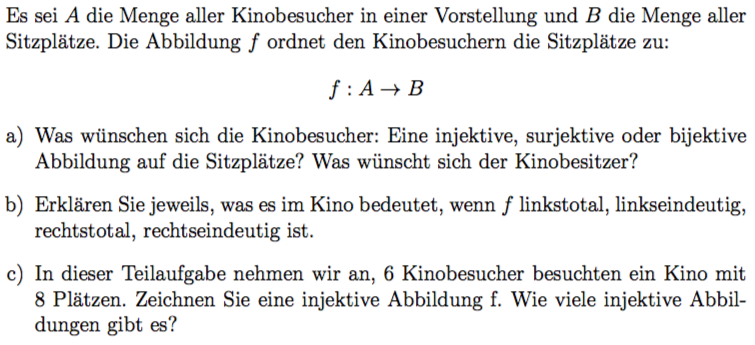
\includegraphics[width=\textwidth]{../topics/mengen-relationen-abbildungen/1.png} 
	\end{figure}     
\end{frame}

\begin{frame}{Aufgabe}
\begin{figure}[h!]
		\centering
		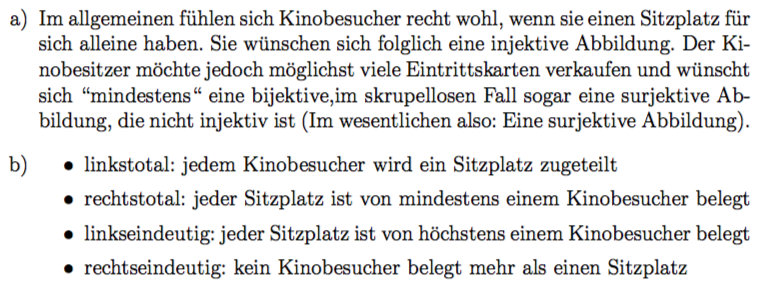
\includegraphics[width=\textwidth]{../topics/mengen-relationen-abbildungen/2.png} 
	\end{figure}  
	\begin{figure}[h!]
		\centering
		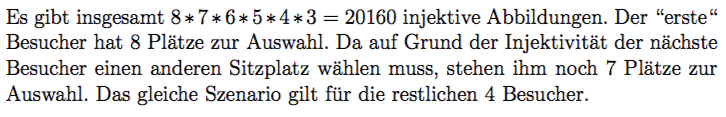
\includegraphics[width=\textwidth]{../topics/mengen-relationen-abbildungen/3.png} 
	\end{figure}   
\end{frame}

\section[ÜB1]{Tipps/Hinweise zum ÜB}
\subsection{ÜB-Tipps}
\begin{frame}{Hinweise zum Übungsblatt}
	\begin{block}{Def.: Notwendige Bedingung}
		Eine \textbf{notwendige Bedingung} zu einer Aussage $K$ ist eine Aussage $A$, für die gilt:

		{\center $K$ kann nur erfüllt sein, wenn die Bedingung $A$ gilt.\\}
		Das heißt \textit{nicht}, dass $K$ erfüllt sein muss.
	\end{block}

	\begin{block}{Def.: Hinreichende Bedingung}
		Eine \textbf{hinreichende Bedingung} zu einer Aussage $K$ ist eine Aussage $B$, für die gilt:
		\center Wenn die Bedingung $B$ erfüllt ist, so ist garantiert auch $K$ erfüllt.
	\end{block}
\end{frame}

%%%%%%%%%% %%%%%%%%%%
%% Zusammenfassung
\section{}
%\subsection{Zusammenfassung}
	\begin{frame}{Was ihr jetzt kennen und können solltet...}
			\begin{itemize}
				%\item Die Begriffe Nachricht, Information und Informationsgehalt mal gehört haben
				\item Die Begriffe Menge, Element einer Menge und set comprehension erklären und ihre Schreibweise kennen
				\item Vereinigung, Schnitt, Differenz, Kardinalität, Potenzmenge von Mengen bilden
				\item Mengengleichheit zeigen
				\item Kartesische Produkte und Relationen explizit schreiben
				\item Eigenschaften von Relationen und Funktionen
			\end{itemize}
	
	\end{frame}
%% Ausblick
%\subsection{Ausblick}
	\begin{frame}{Ausblick}
		\begin{itemize}
			\item Alphabete, Wörter, Sprachen
		\end{itemize}
	\end{frame}
%%%%%%%%%% %%%%%%%%%%
\section{}
\questionframe
\showmessage{Vielen Dank für eure Aufmerksamkeit.\\ Bis zum nächsten Mal!}
%\lastframe
\mode<handout>{\slideThanks}
\end{document}